\begin{figure}[htp]
  \centering
  \begin{tikzpicture}
    \begin{axis}[width=\textwidth, height=6cm, ylabel=Spannung $U$ in \si{\volt}, xlabel=Wellenlänge $\lambda$ in \si{\micro\metre},xmin=1500, xmax=17750, legend cell align={left}, scaled x ticks={real:1000}, xtick scale label code/.code={}]
      \addplot[blue, thick] table[x index=0,y index=1, col sep=semicolon]{Daten/AbsorptionSiO2.csv};
      \addlegendentry{mit Dotierung}
      \addplot[orange, thick] table[x index=0,y index=2, col sep=semicolon]{Daten/AbsorptionSiO2.csv};
      \addlegendentry{ohne Dotierung}
      \addplot[green!50!black, thick] table[x index=0,y index=3, col sep=semicolon]{Daten/AbsorptionSiO2.csv};
      \addlegendentry{Referenz}
    \end{axis}
  \end{tikzpicture}
  \caption{Signale am Thermoelement bei Plättchen mit dotiertem sowie mit undotierten \ce{SiO2} im Strahlengang sowie ohne Plättchen im Strahlengang}
  \label{fig:AbsorptionSiO2}
\end{figure}

% \begin{figure}[htp]
%   \centering
%     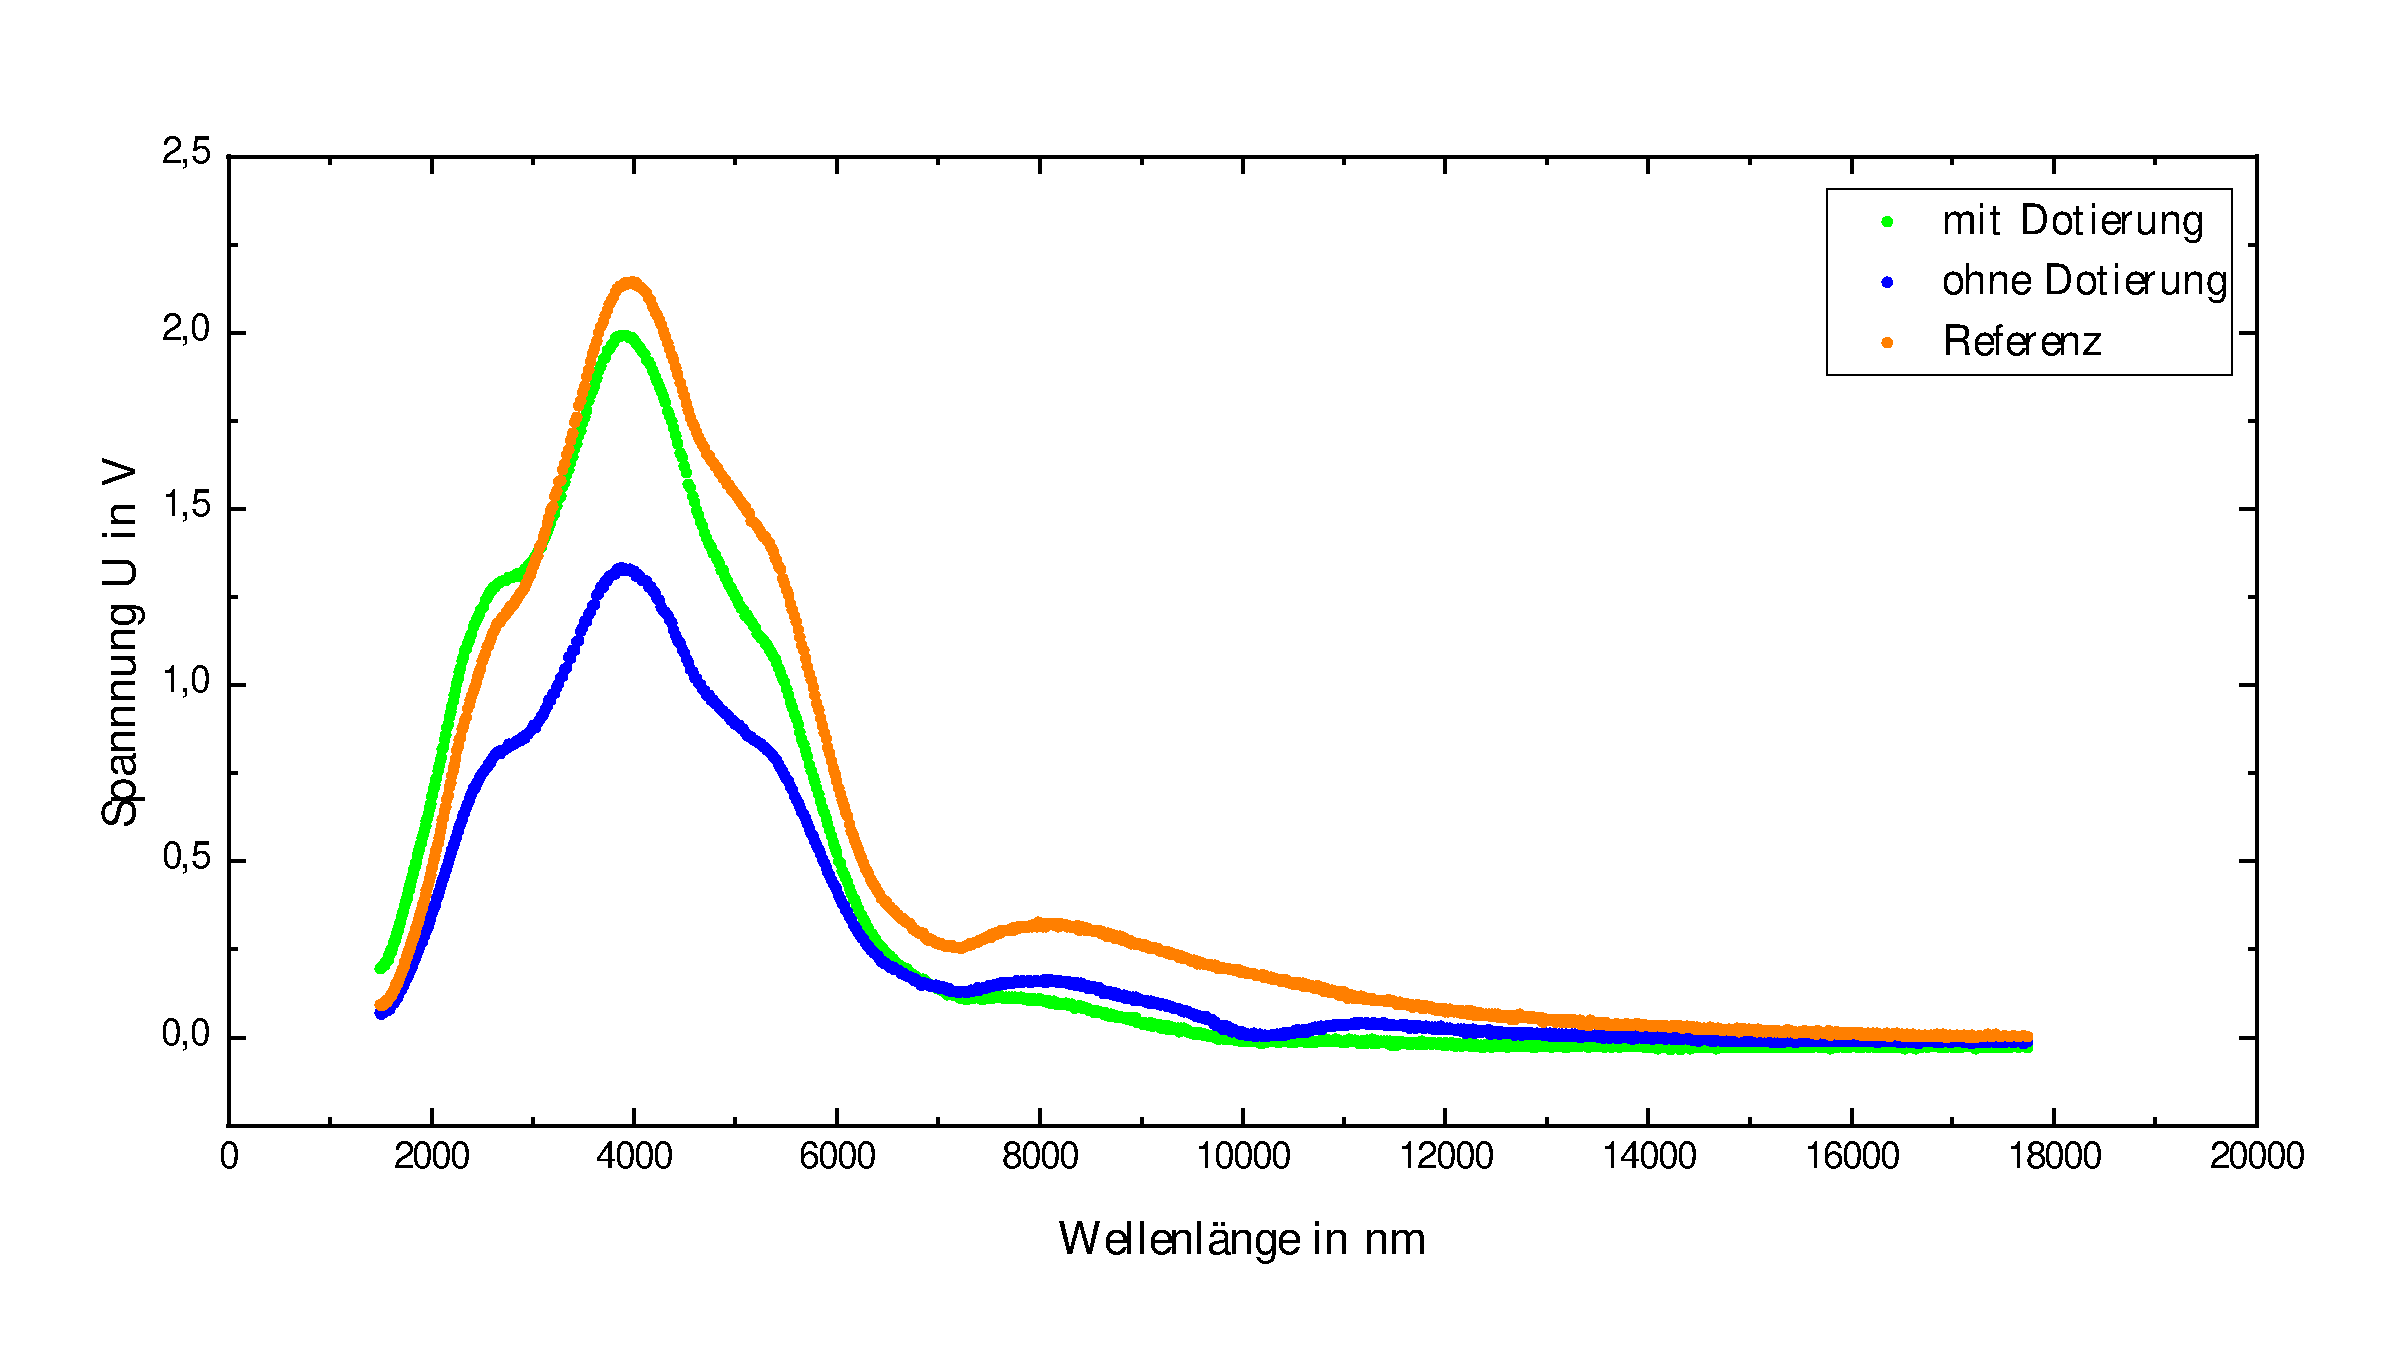
\includegraphics[width=\textwidth]{Bilder/AbsorptionSiO2.pdf}
%     \caption{Signale am Thermoelement bei Plättchen mit dotiertem sowie mit undotierten \ce{SiO2} im Strahlengang sowie ohne Plättchen im Strahlengang}
% \end{figure}
